% Options for packages loaded elsewhere
\PassOptionsToPackage{unicode}{hyperref}
\PassOptionsToPackage{hyphens}{url}
%
\documentclass[
  answers,addpoints,12pt]{exam}
\usepackage{amsmath,amssymb}
\usepackage{lmodern}
\usepackage{iftex}
\ifPDFTeX
  \usepackage[T1]{fontenc}
  \usepackage[utf8]{inputenc}
  \usepackage{textcomp} % provide euro and other symbols
\else % if luatex or xetex
  \usepackage{unicode-math}
  \defaultfontfeatures{Scale=MatchLowercase}
  \defaultfontfeatures[\rmfamily]{Ligatures=TeX,Scale=1}
\fi
% Use upquote if available, for straight quotes in verbatim environments
\IfFileExists{upquote.sty}{\usepackage{upquote}}{}
\IfFileExists{microtype.sty}{% use microtype if available
  \usepackage[]{microtype}
  \UseMicrotypeSet[protrusion]{basicmath} % disable protrusion for tt fonts
}{}
\makeatletter
\@ifundefined{KOMAClassName}{% if non-KOMA class
  \IfFileExists{parskip.sty}{%
    \usepackage{parskip}
  }{% else
    \setlength{\parindent}{0pt}
    \setlength{\parskip}{6pt plus 2pt minus 1pt}}
}{% if KOMA class
  \KOMAoptions{parskip=half}}
\makeatother
\usepackage{xcolor}
\usepackage[top=1.5cm,bottom=1.5cm,left=1.5cm,right=1.5cm]{geometry}
\usepackage{longtable,booktabs,array}
\usepackage{calc} % for calculating minipage widths
% Correct order of tables after \paragraph or \subparagraph
\usepackage{etoolbox}
\makeatletter
\patchcmd\longtable{\par}{\if@noskipsec\mbox{}\fi\par}{}{}
\makeatother
% Allow footnotes in longtable head/foot
\IfFileExists{footnotehyper.sty}{\usepackage{footnotehyper}}{\usepackage{footnote}}
\makesavenoteenv{longtable}
\usepackage{graphicx}
\makeatletter
\def\maxwidth{\ifdim\Gin@nat@width>\linewidth\linewidth\else\Gin@nat@width\fi}
\def\maxheight{\ifdim\Gin@nat@height>\textheight\textheight\else\Gin@nat@height\fi}
\makeatother
% Scale images if necessary, so that they will not overflow the page
% margins by default, and it is still possible to overwrite the defaults
% using explicit options in \includegraphics[width, height, ...]{}
\setkeys{Gin}{width=\maxwidth,height=\maxheight,keepaspectratio}
% Set default figure placement to htbp
\makeatletter
\def\fps@figure{htbp}
\makeatother
\setlength{\emergencystretch}{3em} % prevent overfull lines
\providecommand{\tightlist}{%
  \setlength{\itemsep}{0pt}\setlength{\parskip}{0pt}}
\setcounter{secnumdepth}{-\maxdimen} % remove section numbering
\newlength{\cslhangindent}
\setlength{\cslhangindent}{1.5em}
\newlength{\csllabelwidth}
\setlength{\csllabelwidth}{3em}
\newlength{\cslentryspacingunit} % times entry-spacing
\setlength{\cslentryspacingunit}{\parskip}
\newenvironment{CSLReferences}[2] % #1 hanging-ident, #2 entry spacing
 {% don't indent paragraphs
  \setlength{\parindent}{0pt}
  % turn on hanging indent if param 1 is 1
  \ifodd #1
  \let\oldpar\par
  \def\par{\hangindent=\cslhangindent\oldpar}
  \fi
  % set entry spacing
  \setlength{\parskip}{#2\cslentryspacingunit}
 }%
 {}
\usepackage{calc}
\newcommand{\CSLBlock}[1]{#1\hfill\break}
\newcommand{\CSLLeftMargin}[1]{\parbox[t]{\csllabelwidth}{#1}}
\newcommand{\CSLRightInline}[1]{\parbox[t]{\linewidth - \csllabelwidth}{#1}\break}
\newcommand{\CSLIndent}[1]{\hspace{\cslhangindent}#1}
% \usepackage{exam}

\newcommand{\bquestions}{\begin{questions}}
\newcommand{\equestions}{\end{questions}}
\newcommand{\bsolution}{\begin{solution}}
\newcommand{\esolution}{\end{solution}}
\newcommand{\bparts}{\begin{parts}}
\newcommand{\eparts}{\end{parts}}
\newcommand{\stpart}{\part} % this is absolutely necessary to make new part command
\newcommand{\bsubparts}{\begin{subparts}}
\newcommand{\esubparts}{\end{subparts}}
\newcommand{\stsubpart}{\subpart}

% solution environment is a minipage and cannot support float so, always use "HOLD_position" 
\usepackage{float} % this package is essential for solution with code
% eqnarray is better avoided, most suggestion lead to \align provided in amsmath
% also split is used when there are very long lines of equation
% for different expression of the same equation use line separator \\ and use \notag or \nonumber
\usepackage{eqnarray, amsmath}

% \usepackage{background}
% \usepackage{eso-pic}
% \usepackage{contour}
% 
% \backgroundsetup{
%   angle=90,
%   opacity=0.8,
%   scale=1.2,
%   color=red,
%   nodeanchor=south west,
%   position={current page.south east},
%   contents={}{{\footnotesize Generated by }{\Large Deependra Dhakal }{(\footnotesize to be shared and distributed freely!)}},
%   hshift=40pt,% to move the text vertically
%   vshift=+10pt% to move the text horizontally
% }
% 
% \pagestyle{empty}

\newcommand{\under}[1]{%
  \vphantom{#1}%
  \underaccent{\bar}{\smash[b]{#1}}%
  }

\newcommand{\probP}{\text{I\kern-0.12em P}}
\usepackage{wasysym}
\usepackage{tikz}
\usetikzlibrary{positioning,decorations.pathreplacing,shapes}
\usepackage{amsmath}
\DeclareMathOperator{\p}{p}
\newcommand{\testp}{\text{test}+}
\usepackage{accents}
\usepackage{epsdice}
\usepackage{pst-poker}
\ifLuaTeX
  \usepackage{selnolig}  % disable illegal ligatures
\fi
\IfFileExists{bookmark.sty}{\usepackage{bookmark}}{\usepackage{hyperref}}
\IfFileExists{xurl.sty}{\usepackage{xurl}}{} % add URL line breaks if available
\urlstyle{same} % disable monospaced font for URLs
\hypersetup{
  pdftitle={Counting, probability, conditional probability and Bayes},
  hidelinks,
  pdfcreator={LaTeX via pandoc}}

\title{Counting, probability, conditional probability and Bayes}
\usepackage{etoolbox}
\makeatletter
\providecommand{\subtitle}[1]{% add subtitle to \maketitle
  \apptocmd{\@title}{\par {\large #1 \par}}{}{}
}
\makeatother
\subtitle{Numerical Exercises}
\author{Deependra Dhakal}
\date{}

\begin{document}
\maketitle

Before delving into this random ocean of numerical problem and solutions, note that several ideas were borrowed from following wonderful references:

\begin{enumerate}
\def\labelenumi{\arabic{enumi}.}
\tightlist
\item
  Khare and Lachowska (2015) (Beautiful, Simple, Exact, Crazy, 2015)
\item
  Angel and Porter (2017) (A survey of mathematics with applications, 2016) -- A higher secondary level mathematics textbook. Contains basic description and problems sets on probability at the final chapters of the book.
\item
  Mills (2014) (Problems in Probability, 2013) -- Chapter 2 has notes and advanced problems on probability. Book comes with solution (at the end) of all chapters.
\item
  Principles of uncertainty, 2011 -- Finely written \textasciitilde500 pages book. Has R codes in-text and several case specific problems and discussion.
\item
  Probability and statistical inference
\item
  Statistics for Engineering and the Sciences, 2016 (with sm)
\item
  Applied probability, 2003 -- Introduces genetics and population genetics concepts at the beginning and nicely relates to probabilistic thinking.
\item
  Mathematical and Statistical Methods for Genetic Analysis, 2002
\item
  Biocalculus Calculus, Probability, and Statistics for the Life Sciences, 2016 (with sm)
\item
  Fundamentals of Biostatistics by Bernard Rosner, 2010
\item
  Biostatistics for Biomedical Research, 2018 (by Frank Harrell)
\item
  Mathematical Models in Biology, 2003 (with sm)
\item
  Introduction to Mathematical Statistics, 6th Edition, 2005 (with sm)
\item
  Mario Lefebvre - Applied Probability and Statistics-Springer, 2006 (with sm)
\item
  Introduction to the Practice of Statistics (6th Edition), 2007 (with sm)
\item
  Introduction to Probability, 2nd Edition, 2008 (with sm)
\item
  Probability, Statistics, and Random Processes For Electrical Engineering, 3rd Edition, 2008 (with sm)
\item
  Probability and Statistical Inference, 8th Edition, 2010 (with sm)
\item
  Engineering Mathematics, Problems and Solutions, Volume I, 2012 -- It is a worked out solution book
\item
  Introduction to Probability with Statistical Applications-Birkhauser Basel, 2016 (with sm)
\item
  Probability and Statistics\_9th Edition, 2016 (with sm)
\item
  Statistics for Engineering and the Sciences, Sixth Edition, 2017 (with sm)
\item
  Introduction to Probability, 2nd Edition, 2019 (Blitzstein J.K., Hwang J.) (with sm)
\item
  Mathematics and Statistics for Science\_Springer, 2022 (with sm)
\end{enumerate}

\hypertarget{permutation}{%
\section{Permutation}\label{permutation}}

\bquestions

\question \label{quest:perm-1}

If you have 15 shirts and 8 pair of pants, how many outfits can you make ?

\bsolution (Question \ref{quest:perm-1})

Since an outfit must consist of a shirt AND a pant, we can get: \(15 \times 8 = 120\) outfits.

\esolution

\question \label{quest:perm-2}

How many three digit numbers have only even digits ?

\bsolution (Question \ref{quest:perm-2})

Let us represent three digit numbers with: \(\under{x}\under{y}\under{z}\).

Then for \(x\), we can have \(\{2,4,6,8\}\) to choose from \(\Longrightarrow\) 4 digits,

For both \(y\) and \(z\), we have \(\{0, 2, 4, 6, 8\}\) to choose from \(\Longrightarrow\) 5 digits.

\(\therefore\) Total numbers that could be made (by arrangements of available digits): \(4 \times 5 \times 5 = 100\).

\esolution

\question \label{quest:perm-3}

\bsolution (Question \ref{quest:perm-3})

\esolution

\question \label{quest:perm-4}

\bsolution (Question \ref{quest:perm-4})

\esolution

\equestions

\hypertarget{probability-conditional-probability-and-bayes}{%
\section{Probability, conditional probability and Bayes}\label{probability-conditional-probability-and-bayes}}

\hypertarget{solved-problems}{%
\subsection{Solved problems}\label{solved-problems}}

\bquestions

\question \label{quest:sample-space-1}

Three different people are to be selected at random, and each will be given one gift card. There is one card from Home Depot, one from Best Buy, and one from Red Lobster. The first person selected gets to choose one of the cards. The second person selected gets to choose between the two remaining cards. The thirds person selected gets the third card.

\begin{enumerate}
\def\labelenumi{\alph{enumi}.}
\tightlist
\item
  If each card is equally likely to be selected, determine the number of sample points in the sample space.
\item
  Determine the probability that the Best Buy card is selected first.
\item
  The cards are selected in the order: Best Buy, Red Lobster, Home Depot.
\end{enumerate}

\bsolution (Question \ref{quest:sample-space-1})

Let the abbreviations Ho, Be and Re represent gift cards respectively from Home Depot, one from Best Buy, and one from Red Lobster. Gift cards could be selected by 3 persons consecutively in: \(3\times 2\times 1\) way. Thus, following possible outcomes are possibles

\(\{Ho,Be,Re\}\), \(\{Ho,Be,Re\}\),
\(\{Re,Be,Ho\}\), \(\{Re,Ho,Be\}\),
\(\{Be,Ho,Re\}\), \(\{Be,Re,Ho\}\).

Total of 6 sample points are possible.

\begin{itemize}
\tightlist
\item
  Out of 6 total outcomes from sample space, 2 of them have \(Be\) selected at first. Hence the probability is \(\frac{2}{6} = \frac{1}{3}\).
\item
  Exactly 1 of the outcomes of the sample space has the cards selected in the order \(\{Be, Re, Ho\}\). Hence the probability is \(\frac{1}{6}\).
\end{itemize}

\esolution

\question \label{quest:sample-space-2}

A single die is rolled twice.

\begin{enumerate}
\def\labelenumi{\alph{enumi}.}
\tightlist
\item
  Determine the number of sample points in the sample space.
\item
  Construct a tree diagram and list the sample space.
\item
  Probability that a double (a 1, 1 or 2, 2, etc.) is rolled.
\item
  Probability that a sum of 8 is rolled.
\item
  Probability that a sum of 2 is rolled.
\item
  Are you as likely to roll a sum of 2 as you are of rolling a sum of 8 ?
\end{enumerate}

\bsolution (Question \ref{quest:sample-space-2})

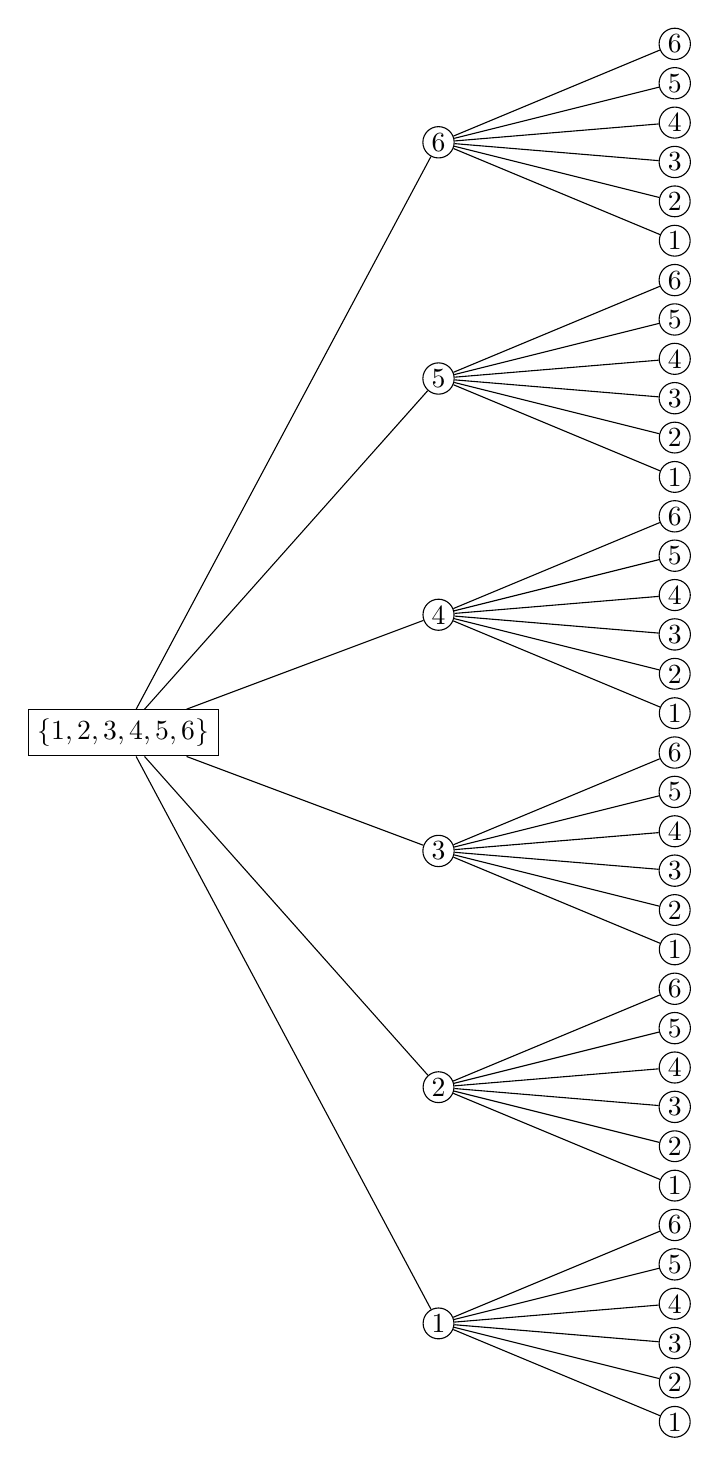
\begin{tikzpicture}[
  grow=right,
  sloped,
  level 1/.style={level distance=4cm,sibling distance=30mm},
  level 2/.style={level distance=3cm,sibling distance=5mm},
  shape=circle,
  rolls/.style={draw, inner sep=1pt, text centered},
]
  \node[draw, rectangle] {$\{ \epsdice{1}, \epsdice{2}, \epsdice{3}, 
          \epsdice{4}, \epsdice{5}, \epsdice{6} \}$} child foreach \i in {1,...,6}
        { node[rolls] {\i} child foreach \i in {1,...,6}
            { node[rolls] {\i}
            }
        };
\end{tikzpicture}

\esolution

\question \label{quest:odds-1}

One card is selected from a standard deck of cards. Determine

\begin{enumerate}
\def\labelenumi{\alph{enumi}.}
\tightlist
\item
  the odds in favor of selecting a queen
\item
  the odds against selecting a queen
\end{enumerate}

\bsolution (Question \ref{quest:odds-1})

There are 52 cards in a standard deck of cards, 4 of which are queens. Therefore, the probability of selecting a queen is \(\frac{4}{52}\), or \(\frac{1}{13}\). The probability the card selected is not a queen is \(1-\frac{1}{13} = \frac{12}{13}\).

Odds in favor of selecting a queen = \(\frac{P(\text{Selecting a queen})}{P(\text{Not selecting a queen})} = \frac{1/13}{12/13} = \frac{1}{12}\) \(\implies\) \(1:12\).

The odds against selecting a queen are \(12:1\).

\esolution

\question \label{quest:iids-1}

(Independent events) Suppose you draw two cards randomly from a deck. Let \(A\) denote the event that the first card is a \(\diamondsuit\), and B that the second card is a \(\diamondsuit\). Are events A and B independent ?

\bsolution (Question \ref{quest:iids-1})

Clearly, \(P(A) = \frac{13}{52} = \frac{1}{4}\). Also, \(P(B)= \frac{1}{4}\). Now we compute \(P(A\cap B)\). This is the event that both cards are diamonds, and its probability is:

\[
P(A \cap B) = \frac{{13\choose 2}}{{52 \choose2}} = \frac{13\times 12}{52\times 51} = \frac{12}{4\times 51} = \frac{1}{17}.
\]

Here, \(n \choose k\) symbol \(\implies\) ``Choose \(k\) items to compose unordered collection of items from \(n\) items''.

On the other hand,

\[
P(A).P(B) = \frac{1}{4}.\frac{1}{4} = \frac{1}{16}.
\]

Therefore, \(P(A). P(B) \neq P(A\cap B)\), and the events are not independent.

\esolution

\question \label{quest:prob-1}

If 5 coins are tossed together, determine the probability of getting

\begin{enumerate}
\def\labelenumi{\arabic{enumi}.}
\tightlist
\item
  3H and 2T
\item
  At least 3H
\item
  More than 3H
\item
  Less than 3H
\item
  Not more than 3H
\end{enumerate}

\bsolution (Question \ref{quest:prob-1})

Let \(a\) represent probability of turning head (\(P(H) = \frac{1}{2}\)) and \(b\) represent the probability of turning tail (\(P(T) = \frac{1}{2}\)), then, Binomial expansion can be used to mimic all 5 tosses.

\[
(a + b)^5 = a^5 + 5a^4b + 10 a^3 b^2 + 10 a^2 b^3 + 5 ab^4 + b^5
\]

Now,

\begin{enumerate}
\def\labelenumi{\arabic{enumi}.}
\tightlist
\item
  Probability(P) of 3H and 2T is given by \(\mathrm{3^{rd}}\) term, which is: \(10 a^3 b^2\) equals \(\frac{5}{16}\).
\item
  Probabilities of having (3H or 4H or 5H)
\item
  Probabilities of having (4H or 5H)
\item
  Probabilities of having (1H or 2H)
\item
  Probabilities of having (1H or 2H or 3H)
\end{enumerate}

\esolution

\question \label{quest:prob-5}

1\% of women at age forty who participate in routine screening have breast cancer. 80\% of women with breast cancer will get positive mammographies. 9.6\% of women without breast cancer will also get positive mammographies. A woman in this age group had a positive mammography in a routine screening. What is the probability that she actually has breast cancer?

\bsolution (Question \ref{quest:prob-5})

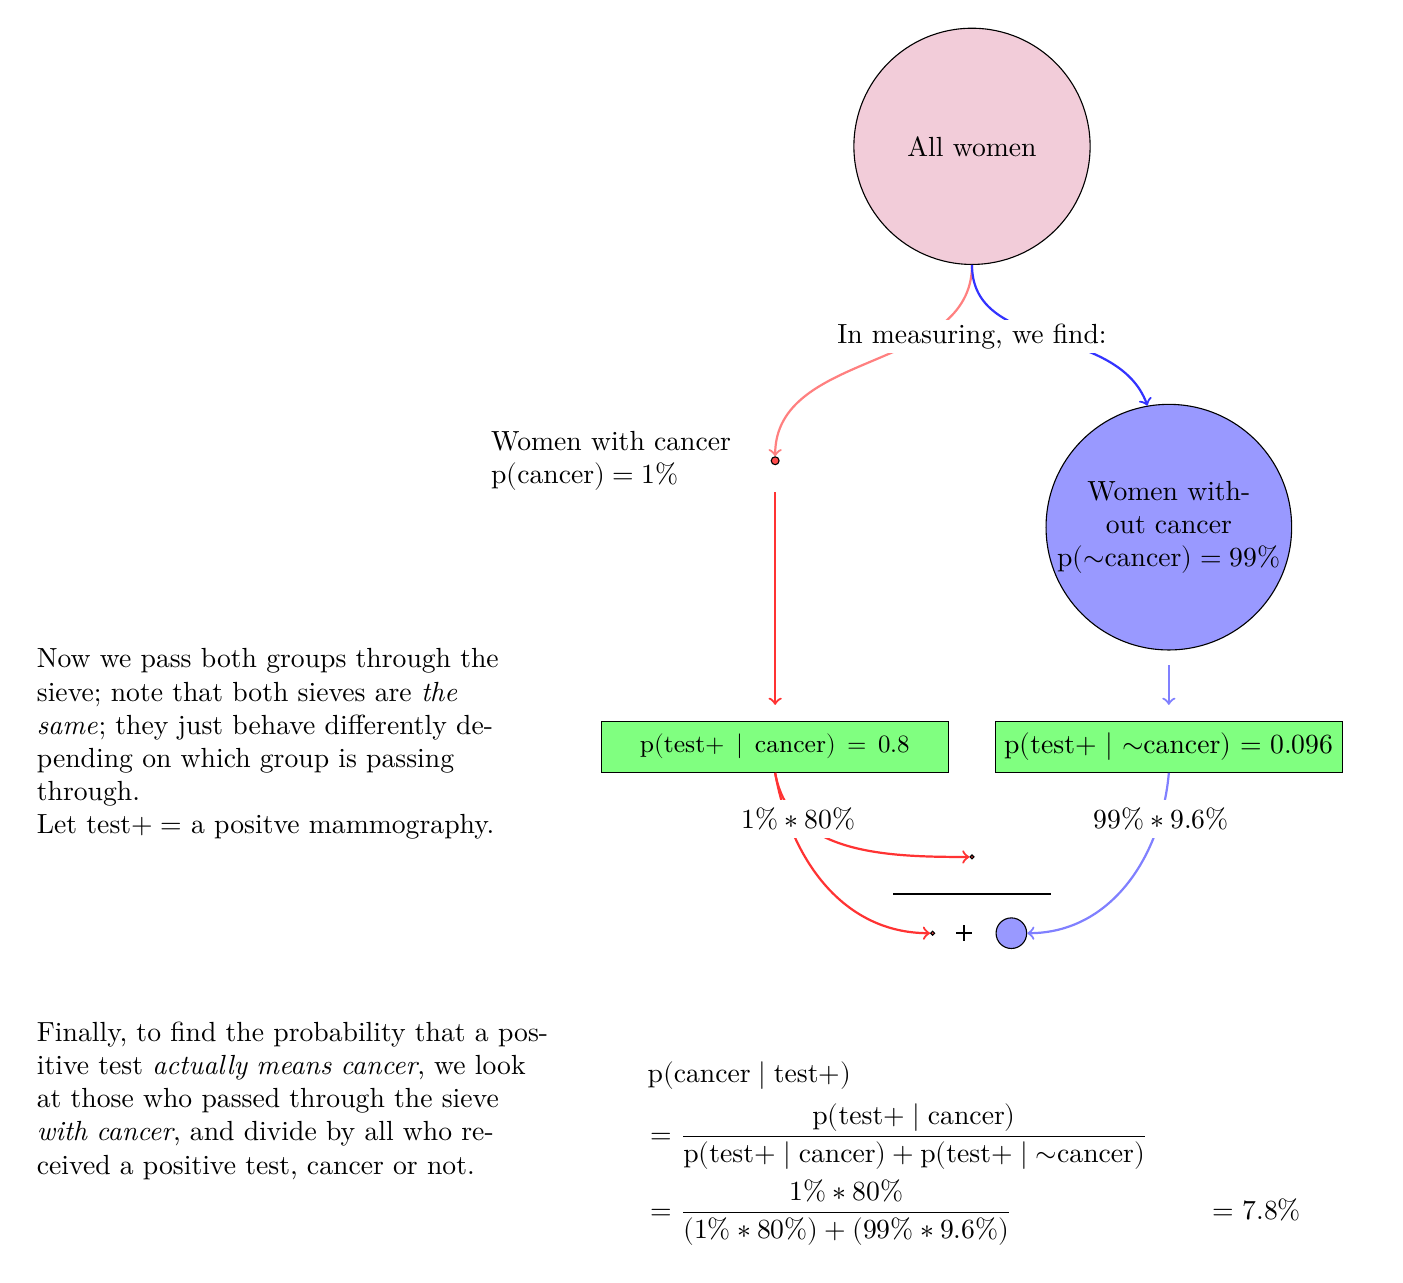
\begin{tikzpicture}[%
  % common options for blocks:
  block/.style = {draw, fill=blue!30, align=center, anchor=west,
              minimum height=0.65cm, inner sep=0},
  % common options for the circles:
  ball/.style = {circle, draw, align=center, anchor=north, inner sep=0}]

% circle illustrating all women
\node[ball,text width=3cm,fill=purple!20] (all) at (6,0) {All women};

% two circles showing split of p{cancer} and p{~cancer}
\node[ball,fill=red!70,text width=0.1cm,anchor=base] (pcan) at (3.5,-5.5) {};
\node[ball,fill=blue!40,text width=2.9cm,anchor=base] (pncan) at (8.5,-6)
   {Women without cancer\\
    $\p({\sim}\text{cancer}) = 99\%$};

% arrows showing split from all women to cancer and ~cancer
\draw[->,thick,draw=red!50] (all.south) to [out=270,in=90] (pcan.north);
\draw[->,thick,draw=blue!80] (all.south) to [out=270,in=110] (pncan.100);

% transition from all women to actual cancer rates
\node[anchor=north,text width=10cm,inner sep=.05cm,align=center,fill=white]
  (why1) at (6,-3.7) {In measuring, we find:};

% note illustration the p{cancer} circle (text won't fit inside)
\node[inner sep=0,anchor=east,text width=3.3cm] (note1) at (3.2,-5.5) {
   Women with cancer $\p(\text{cancer}) = 1\%$};

% draw the sieves
\node[block,anchor=north,text width=4.4cm,fill=green!50] (tray1) at
   (3.5,-8.8) {\small{$\p(\testp\mid\text{cancer})=0.8$}};

\node[block,anchor=north,text width=4.4cm,fill=green!50] (tray2) at
   (8.5,-8.8) {$\p(\testp\mid{\sim}\text{cancer})=0.096$};

% text explaining how p{cancer} and p{~cancer} behave as they
% pass through the sieves
\node[anchor=west,text width=6cm] (note1) at (-6,-9.1) {
   Now we pass both groups through the sieve; note that both
     sieves are \emph{the same}; they just behave differently
     depending on which group is passing through. \\ 
     Let $\testp=$ a positve mammography.};

% arrows showing the circles passing through the seives
\draw[->,thick,draw=red!80] (3.5,-5.9) -- (3.5,-8.6);
\draw[->,thick,draw=blue!50] (8.5,-8.1) -- (8.5,-8.6);

% numerator
\node[ball,text width=0.05cm,fill=red!70] (can) at (6,-10.5) {};

% dividing line
\draw[thick] (5,-11) -- (7,-11);

% demoniator
\node[ball,text width=0.39cm,fill=blue!40,anchor=base] (ncan) at (6.5,-11.5) {};
\node[ball,text width=0.05cm,fill=red!70,anchor=base] (can2) at (5.5,-11.5) {};

% plus sign in denominator
\draw[thick] (5.9,-11.4) -- (5.9,-11.6);
\draw[thick] (5.8,-11.5) -- (6,-11.5);

% arrows showing the output of the sieves formed the fraction
\draw[->,thick,draw=red!80] (tray1.south) to [out=280,in=180] (can);
\draw[->,thick,draw=red!80] (tray1.south) to [out=280,in=180] (can2);
\node[anchor=north,inner sep=.1cm,align=center,fill=white] (why2) at
   (3.8,-9.8) {$1\% * 80\%$};

\draw[->,thick,draw=blue!50] (tray2.south) to [out=265,in=0] (ncan);
\node[anchor=north,inner sep=.1cm,align=center,fill=white] (why2) at
   (8.4,-9.8) {$99\% * 9.6\%$};

% explanation of final formula
\node[anchor=north west,text width=6.5cm] (note2) at (-6,-12.5)
   {Finally, to find the probability that a positive test
       \emph{actually means cancer}, we look at those who passed
       through the sieve \emph{with cancer}, and divide by all who
       received a positive test, cancer or not.}; 

% illustrated fraction turned into math
\node[anchor=north,text width=10cm] (solution) at (6,-12.5) {
  \begin{align*}
    & \p(\text{cancer}\mid\testp) & \\
    & =\frac{\p(\testp\mid\text{cancer})}{\p(\testp\mid\text{cancer})
        + \p(\testp\mid{\sim}\text{cancer})} & \\
    & =\frac{1\% * 80\%}{(1\% * 80\%) + (99\% * 9.6\%)} &= 7.8\%
   \end{align*}};
\end{tikzpicture}

\esolution

\question \label{quest:prob-6}

Suppose that a barrel contains many small plastic eggs. Some eggs are painted red and some are painted blue. 40\% of the eggs in the bin contain pearls, and 60\% contain nothing. 30\% of eggs containing pearls are painted blue, and 10\% of eggs containing nothing are painted blue. What is the probability that a blue egg contains a pearl?

\bsolution (Question \ref{quest:prob-6})

We have,

\(\probP(\text{pearl}) = 40\%\)

\(\probP(\text{blue}|\text{pearl}) = 30\%\)

\(\probP(\text{blue}|\sim{}\text{pearl}) = 10\%\)

\(\probP(\text{pearl}|\text{blue}) = ?\)

It can be learnt that,

\begin{itemize}
\tightlist
\item
  Since 40\% of the eggs contain pearls and 30\% of the eggs containing pearls are painted blue, 12\% of the eggs altogether contain pearls and are painted blue.
\item
  Since 60\% of the eggs contain nothing and 10\% of the eggs containing nothing are painted blue, 6\% of the eggs contain nothing and are painted blue.
\item
  A total of 18\% (12 + 6) of the eggs are painted blue.
\end{itemize}

\(\therefore\) \(\probP(\text{pearl}|\text{blue}) = \frac{\probP(\text{perl}) \land \probP(\text{blue})}{\probP (\text{blue})} = \frac{12}{18}\)

\esolution

\question \label{quest:prob-7}

Suppose we draw a card and it turns out to be red. What are the odds that the card is a \(\diamondsuit\) ?

\bsolution (Question \ref{quest:prob-7})

Let \(A\) denote getting a diamond and B getting a red card. Then \(\probP(A\cap B)\) is the probability that a card is red and a diamond, which simply means that it is a diamond, \(\probP(A\cap B) = 1/4\). The probability of a card being red is \(\probP(B) = 1/2\). Therefore, the probability of a card being a diamond, given that it is red, is:

\[
\probP (A|B) = \frac{\probP(A\cap B)}{\probP(B)} = \frac{1/4}{1/2} = 1/2.
\]

\esolution

\question \label{quest:prob-8}

Rolling three dice, what is the probability of getting a \(\epsdice{3}\) on the first roll if the sum of the three outputs is 6 ?

\bsolution (Question \ref{quest:prob-8})

Let \(A\) denote the even that the sum of the three outputs is 6, and \(B\) the event of getting a 3 on the first roll. We need to find \(P(B|A)\). By definition,

\[
P(B|A) = \frac{P(A \cap B)}{P(A)}
\]

The outcomes in A are \(\{\epsdice{2},\epsdice{2},\epsdice{2}\}\), \(\{\epsdice{1},\epsdice{1},\epsdice{4}\}\), \(\{\epsdice{4},\epsdice{1},\epsdice{1}\}\), \(\{\epsdice{1},\epsdice{4},\epsdice{1}\}\), and the six permutations of \(\{1,2,3\}\), totalling ten outcomes. (\(\because~ _3P_3 = 3! = 6\).) Then we have \(P(A) = \frac{10}{6^3} = \frac{5}{108}\). The outcomes of \((A \cap B)\) are \(\{3,2,1\}\) and \(\{3,1,2\}\), so \(P(A\cap B) = \frac{2}{6^3} = \frac{1}{108}\). Then

\[
\large
P(B|A) = \frac{\frac{1}{108}}{\frac{5}{108}} = \frac{1}{5}.
\]

We could have used Bayes' law to compute the same probability:

\[
P(B|A) = \frac{P(A|B).P(B)}{P(A)}.
\]

Then we need to know \(P(B)\) and \(P(A|B)\). The first is easy: the probability of getting a 3 in one roll of a die is \(P(B) = \frac{1}{6}\). The second is the probability of getting the sum of the three outputs equal to 6, given that the first output is \(\epsdice{3}\). This is the same as the probability of getting the sum of two outputs in two rolls equal to 3. There are two possibilities: \(\{1,2\}\) and \(\{2,1\}\). Therefore, \(P(A|B) = \frac{2}{36} = \frac{1}{18}\). Bayes' law gives

\[
P(B|A) = \frac{P(A|B).P(B)}{P(A)} = \frac{\frac{1}{18}.\frac{1}{6}}{\frac{5}{108}} = \frac{1}{5}.
\]

\esolution

\question \label{quest:prob-9}

\bsolution (Question \ref{quest:prob-9})

\esolution

\equestions

\hypertarget{refs}{}
\begin{CSLReferences}{1}{0}
\leavevmode\vadjust pre{\hypertarget{ref-angel2017survey}{}}%
Angel, Allen R, and Stuart R Porter. 2017. \emph{A Survey of Mathematics with Applications}. Pearson Addison Wesley.

\leavevmode\vadjust pre{\hypertarget{ref-khare2015beautiful}{}}%
Khare, Apoorva, and Anna Lachowska. 2015. \emph{Beautiful, Simple, Exact, Crazy}. Yale University Press.

\leavevmode\vadjust pre{\hypertarget{ref-mills2014problems}{}}%
Mills, TM. 2014. \emph{Problems in Probability}. Vol. 13. World Scientific.

\end{CSLReferences}

\end{document}
